\documentclass{tudelft-report}

% 1)Translates MATLAB code:
\usepackage[framed,numbered,autolinebreaks,useliterate]{mcode}
% enclose the MATLAB code by using begin/end{lstlisting}

% 2)Multiple figures on one page
\usepackage{float}
\usepackage{graphicx}
\usepackage{amsmath}
\usepackage{amssymb}
\usepackage{wasysym}
\usepackage{subcaption}
\usepackage{multirow}
\usepackage{caption}
\usepackage{subcaption}
% 3)


\begin{document}

%% Use Roman numerals for the page numbers of the title pages and table of
%% contents.
\frontmatter

\title[Exploiting comments for personalized recommendations]{Where will you comment next?}
\author{P.S.N. Chandrasekaran Ayyanathan}
\affiliation{Faculty of Computer Science}

%\coverimage{cover.jpg}
\makecover[backboxheight = 2.64in]


%% Include an optional title page.
\begin{titlepage}

\begin{center}

%% Insert the TU Delft logo at the bottom of the page.
\begin{tikzpicture}[remember picture,overlay]
    \node at (current page.south)[anchor=south,inner sep=0pt]{
        
\includegraphics{cover/logo}
    };
\end{tikzpicture}

%% Extra whitespace at the top.
\vspace*{2\bigskipamount}

%% Print the title in cyan.
{\makeatletter
\titlestyle\color{tudelft-cyan}\Huge\@title
\makeatother}

%% Print the optional subtitle in black.
{\makeatletter
\ifx\@subtitle\undefined\else
    \bigskip
    \titlefont\titleshape\LARGE\@subtitle
\fi
\makeatother}

\bigskip
\bigskip

by
%door

\bigskip
\bigskip

%% Print the name of the author.
{\makeatletter
\titlefont\Large\bfseries\@author
\makeatother}

\vfill

in partial fulfillment of the requirements for the degree of
%in overeenstemming met de vereisten voor het verkrijgen van de graad van

\bigskip
\bigskip

{\bfseries Master of Science}

in Computer Science

\bigskip
\bigskip

at the Delft University of Technology,
%aan de Technische Universiteit Delft,

to be defended publicly on TBA %Tuesday January 1, 2013 at 10:00 AM.
%in het openbaar de verdedigen op dinsdag 1 januari om 10:00 uur.

\vfill

\begin{tabular}{lll}
%% Add additional information here, per faculty requirements, e.g
%    Student number: & 1234567 \\
%    Project duration: & \multicolumn{2}{l}{March 1, 2012 -- January 1, 2013} \\
    Supervisor: & Prof.\ dr.\ ir.\ M.\ Larson \\
    Thesis committee:
        %& Prof.\ dr.\ C.\ F.\ Xavier, & TU Delft \\
        %& Dr.\ E.\ L.\ Brown, & TU Delft \\
        %& Ir.\ M.\ Scott, & Acme Corporation
\end{tabular}

%% Only include the following lines if confidentiality is applicable.
\bigskip
\bigskip
\emph{This thesis is confidential and cannot be made public until TBA.}
%\emph{Op dit verslag is geheimhouding van toepassing tot en met 31 december 2013.}

\bigskip
\bigskip
An electronic version of this thesis is available at \url{http://repository.tudelft.nl/}.
%Een elektronische versie van dit verslag is beschikbaar op \url{http://repository.tudelft.nl/}.

\end{center}

\end{titlepage}



\chapter*{Abstract}
\setheader{Abstract}
Since the advent of Web 2.0, users have not increasingly created content, but also contributed reactions to content in the form of comments. Comments are challenging to analyze due to their short lengths and informal style, meaning that any individual comment provides very little data to work with and is highly variable. However, comments capture innate and an explicit opinion of a user that makes it invaluable towards personalization. In this work, we explore the possibilities of exploiting comments towards the end of personalized recommendations. We employ state-of-art techniques utilizing this unique form of feedback and evaluate it against the popular Dutch news website NU.nl with results reporting \ldots (TODO)
\chapter*{Preface}
\setheader{Preface}

Preface\ldots

\begin{flushright}
{\makeatletter\itshape
    \@author \\
    Delft, TBA
\makeatother}
\end{flushright}



\tableofcontents

%% Use Arabic numerals for the page numbers of the chapters.
\mainmatter

\chapter{Introduction}
\label{chap:intro}
Everyone has probably had the experience of walking into a restaurant which has a menu that makes no sense and not knowing what to expect would then ask the waiter to recommend some quality dishes that are native to the restaurant. The waiter would then go on to list some of the specialities of the restaurant, some favorites of other customers and to some extent also explain the  meat or flavoring that the dish comprises of. Finally, the customer would then make a decision on what would be appropriate to his own tastes.

Recommender systems are no less different from the waiter of that unfamiliar restaurant. They strive to satisfy the user's needs by providing a quality experience taking his own tastes and interests into account. The core aspect of a recommender is to not pose a user with too much information but only give him what he desires. Recommender systems heavily rely upon user feedback as a form of learning user behaviour and interests. Conventional recommender systems make use of explicit user ratings on items and where ratings are not available, they make use of clicks. For further personalization, clicks are often enriched with meta-data regarding the item, for instance tags. In addition, many web applications do not make use of an explicit `dislike' button as this is often conceived as offending the original author of the item. While there exists a `like' button which in most cases implicates a good recommendation was received, there is no direct way to capture the opposite.

Various forms of meta-data have been extensively studied as forms of user feedback. Ye et al. investigate geo-location awareness enriched upon social networking for recommending new locations \cite{ye_location_2010}.  Castagnos et al. report implications of eye tracking for recommendation in an e-commerce scenario \cite{castagnos_eye-tracking_2010}. Liu et al. move further into the user's body by investigating user's heartbeat as an attribute towards personalized music recommendation \cite{liu_music_2009}. While the rate at which sensors evolve over the years, it is inevitable that this would be the future of recommendations. But, there is a more personal and explicit form of feedback that has been ignored all along. 

Consider the case of a cold state scenario where a new user probes the system and clicks on one of the top recommendations and the user did not like want was presented in the item either because the original title to the item was misleading or he had accidentally clicked on it. In a naive click based recommendation, the user is immediately flooded with similar items. As most web applications often tie the hands of users by not providing explicit `dislike' feedback, they then turn to the only possible way of expressing 
their discontent - comments.

Comments have evolved over the years, initially it was perceived as a form of providing feedback. Now, with introduction of various features such as `upvote/downvote' comments have now become more of a struggle to achieve the most votes through witty opinions or providing genuine additive information. The `reply' feature in comments have also turned commenting platforms into conversational mediums leading to heated debates. In this work, we perform exploratory research into discovering the usefulness of this unique user feedback medium towards personalization in recommendations.

\newpage
\section{Research Flow}
Over the course of our work, we will answer the following research questions. Figure~\ref{fig:r_questions_rep} in essence represents what factors to take into consideration while training the model for our recommender, whereas Figure~\ref{fig:r_questions_pred} represents that of making predictions using our model. Finally, Figure~\ref{fig:r_questions_misc} refers to domain specific questions as we are investigating the particular domain of news recommendation.

\begin{figure}[!h]
\centering
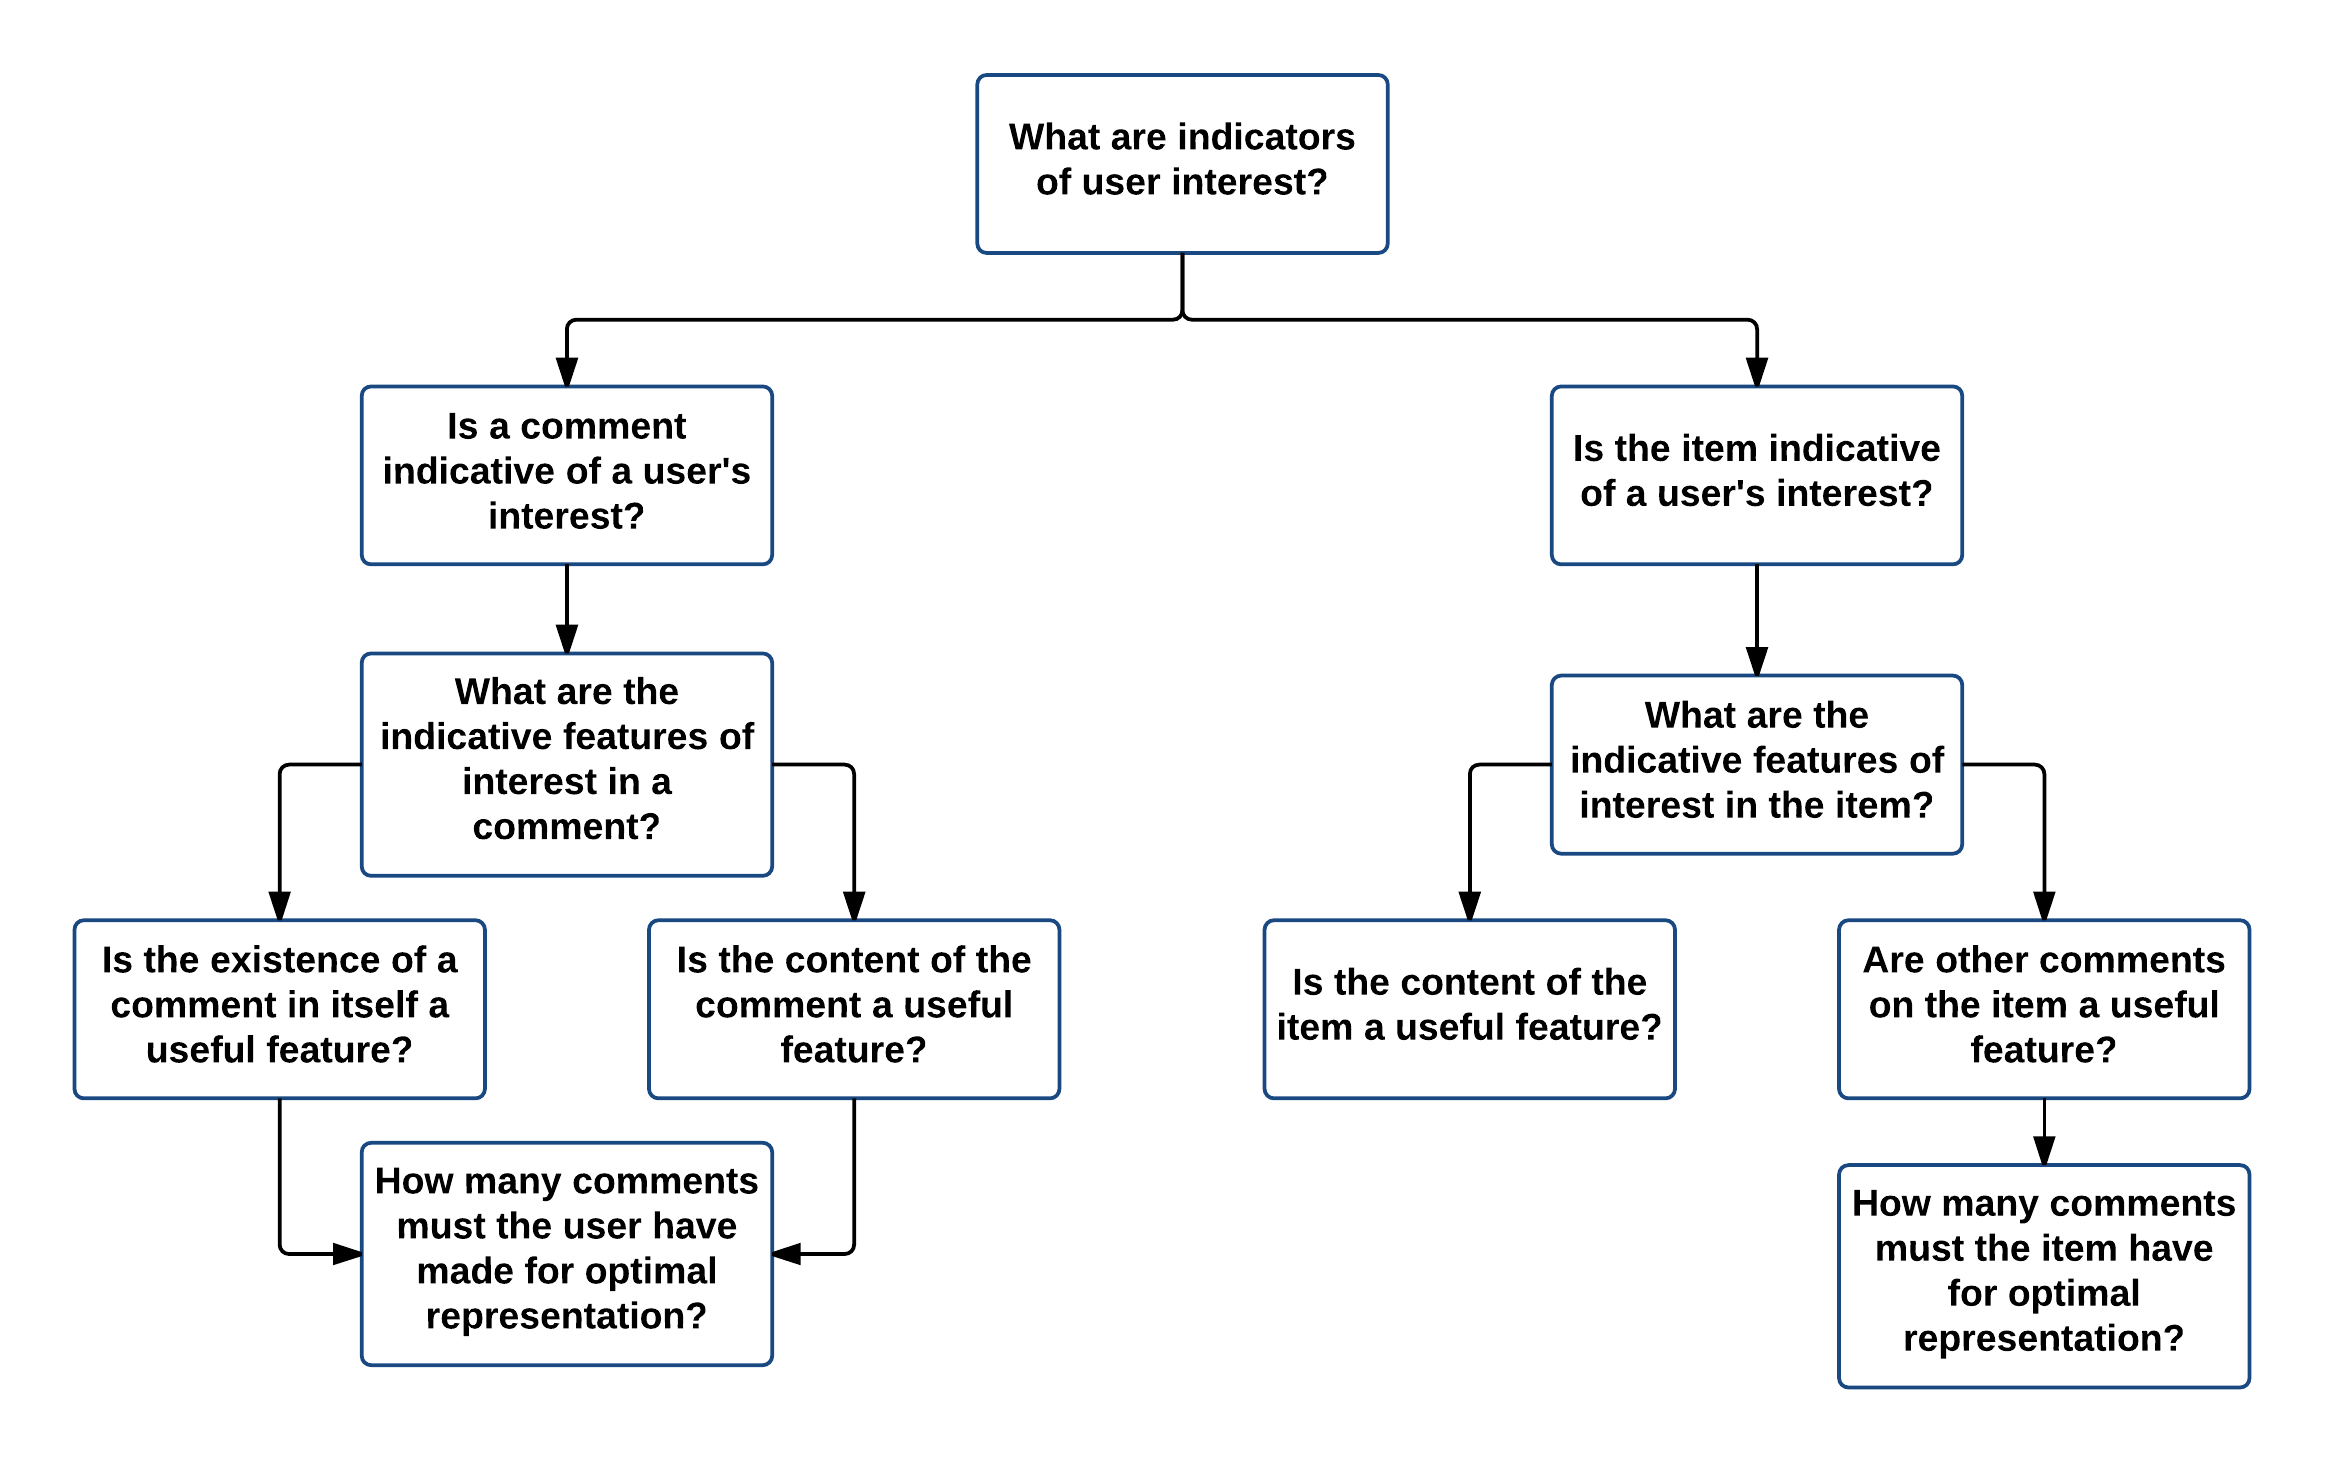
\includegraphics[width=0.905\textwidth]{c-intro_images/r_questions_1.png}
\caption{Representation of Interest}
\label{fig:r_questions_rep}
\end{figure}

\begin{figure}[!h]
\centering
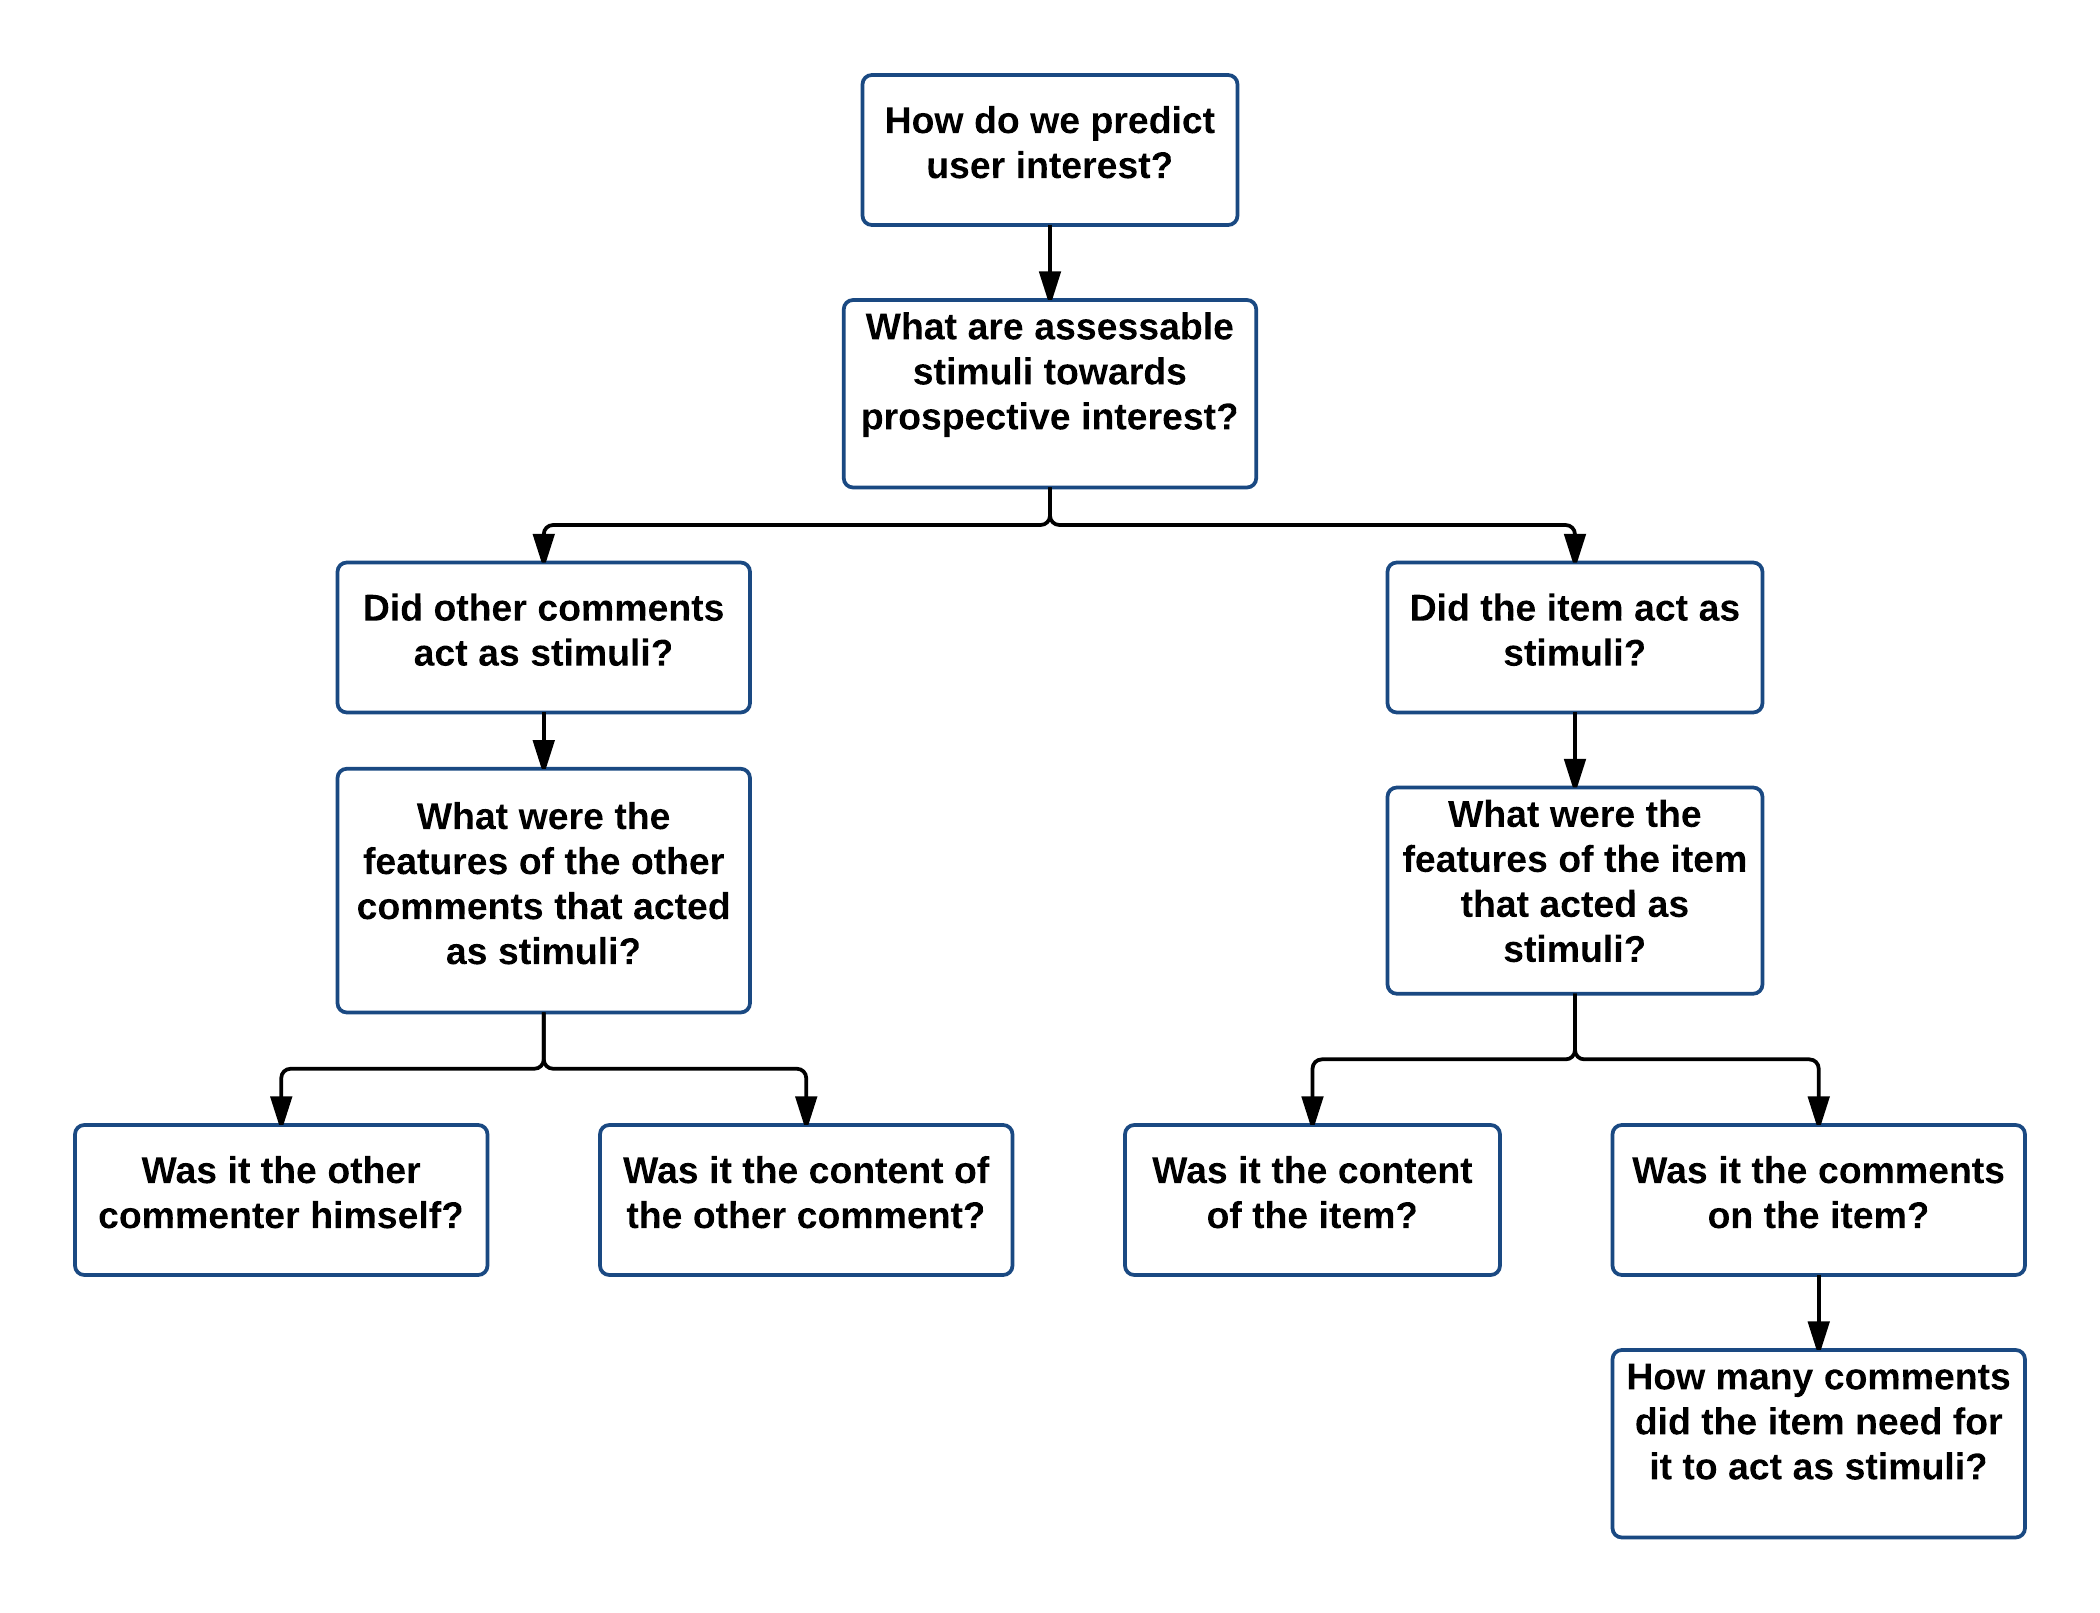
\includegraphics[width=0.8\textwidth]{c-intro_images/r_questions_2.png}
\caption{Prediction of Interest}
\label{fig:r_questions_pred}
\end{figure}

\begin{figure}[!h]
\centering
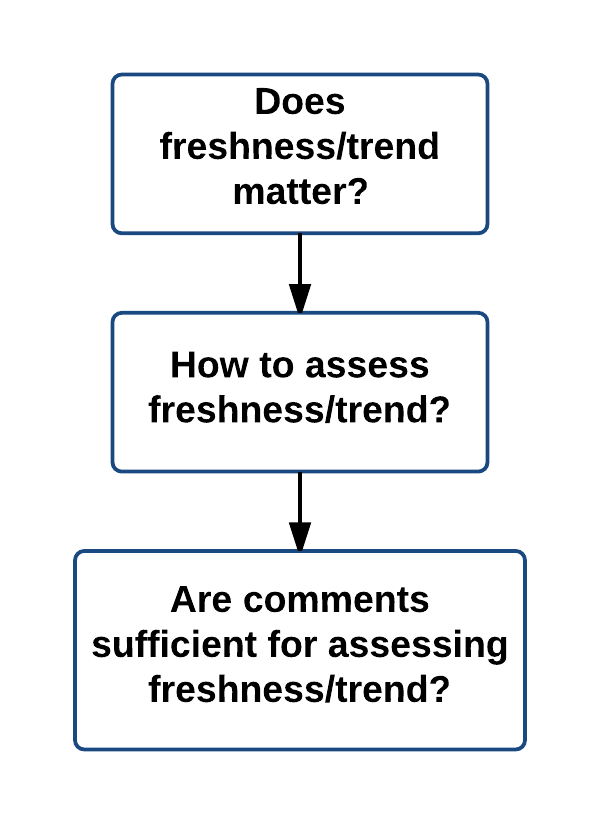
\includegraphics[width=0.25\textwidth]{c-intro_images/r_questions_3.png}
\caption{Domain Specific}
\label{fig:r_questions_misc}
\end{figure}

\section{Related Work (draft)}
Comments have long been under the radar of research, some notable works include the very detailed study of weblog comments by Mishne and Glance \cite{mishne_leave_2006}, summarization of blogs through the comments they receive by Hu et al. \cite{hu_comments-oriented_2008}, popularity prediction of news articles utilizing comments they receive by Tatar et al. \cite{tatar_predicting_2011}, search re-ranking of images through comments by San Pedro et al. \cite{san_pedro_leveraging_2012} and many more. 

In a recommendation scenario, comments are not widely studied. The prominent of the few being recommendation of news stories taking the existence of comments as a form of implicit feedback by Shmueli et al. \cite{shmueli_care_2012} and a more recent work of recommending news stories by also accounting for cold start through the existence of a comment by Saveski and Mantrach \cite{saveski_item_2014}.

So, a clear pattern is observed here, the content of comments have been extensively studied for various information retrieval tasks but have not been employed in a recommendation scenario. In a recommendation scenario, it is only viewed as a form of feedback and only the existence of the comment is only ever taken into consideration. The novelty of our work therein lies to also exploit the content of comments as a means for personalized recommendations.

\section{Thesis Organization? (TODO)}
\chapter{Background}
In this chapter we provide a brief background on recommender systems and their growth over the years.


\section{Recommender Systems}
Recommender systems are essentially glorified information retrieval algorithms. They aim to predict a user's interest towards a web item by utilizing a variety of data ranging from the user's behaviour history to the actual content of the web item. Recommender systems have become a very popular phenomenon and are prevalent in the web, be it electronic retailers such as eBay and Amazon or social networking sites such as Facebook and Twitter, the underlying motivation across domains remains relatively the same - to retain the user on the site by delivering him content he would find interesting.

Earlier we discussed on how different forms of feedback affect recommendations. Now, we briefly discuss the major techniques employed in recommender systems.

\subsection{Collaborative Filtering}
\cite{goldberg_using_1992}
\begin{figure}[!h]
\centering
\begin{subfigure}[b]{0.4\textwidth}
    \centering
    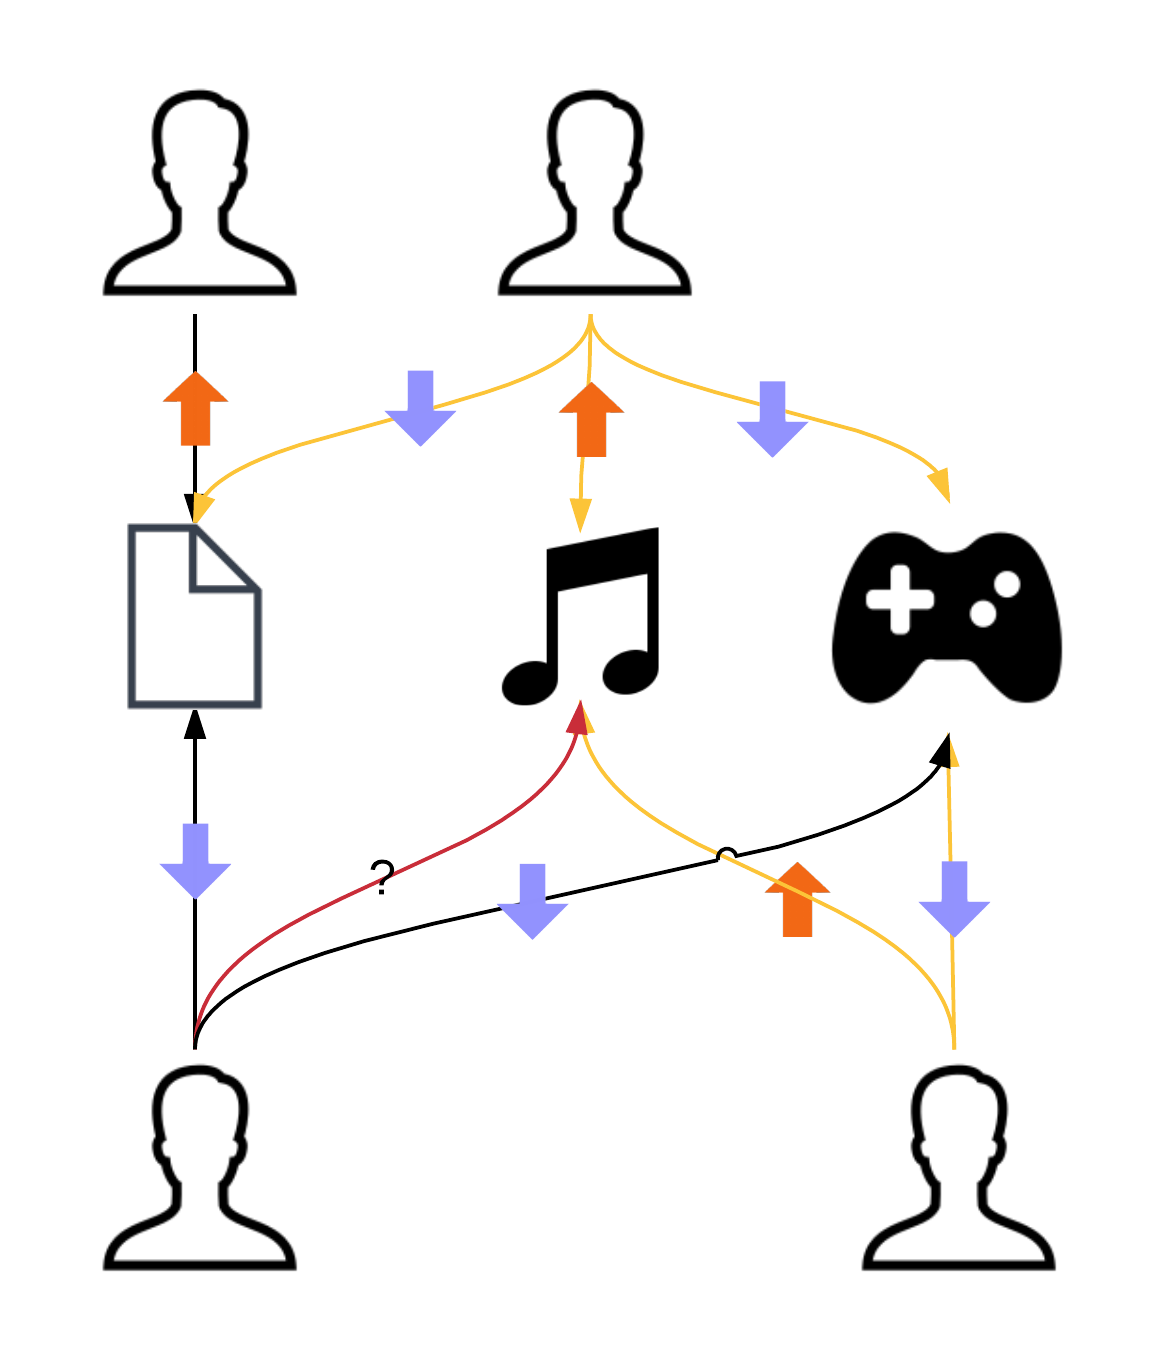
\includegraphics[width=\textwidth]{c-back_images/cf_1.png}
    \caption{Before Prediction}
    \label{fig:cf1}
\end{subfigure}
\hfill
\begin{subfigure}[b]{0.4\textwidth}
    \centering
    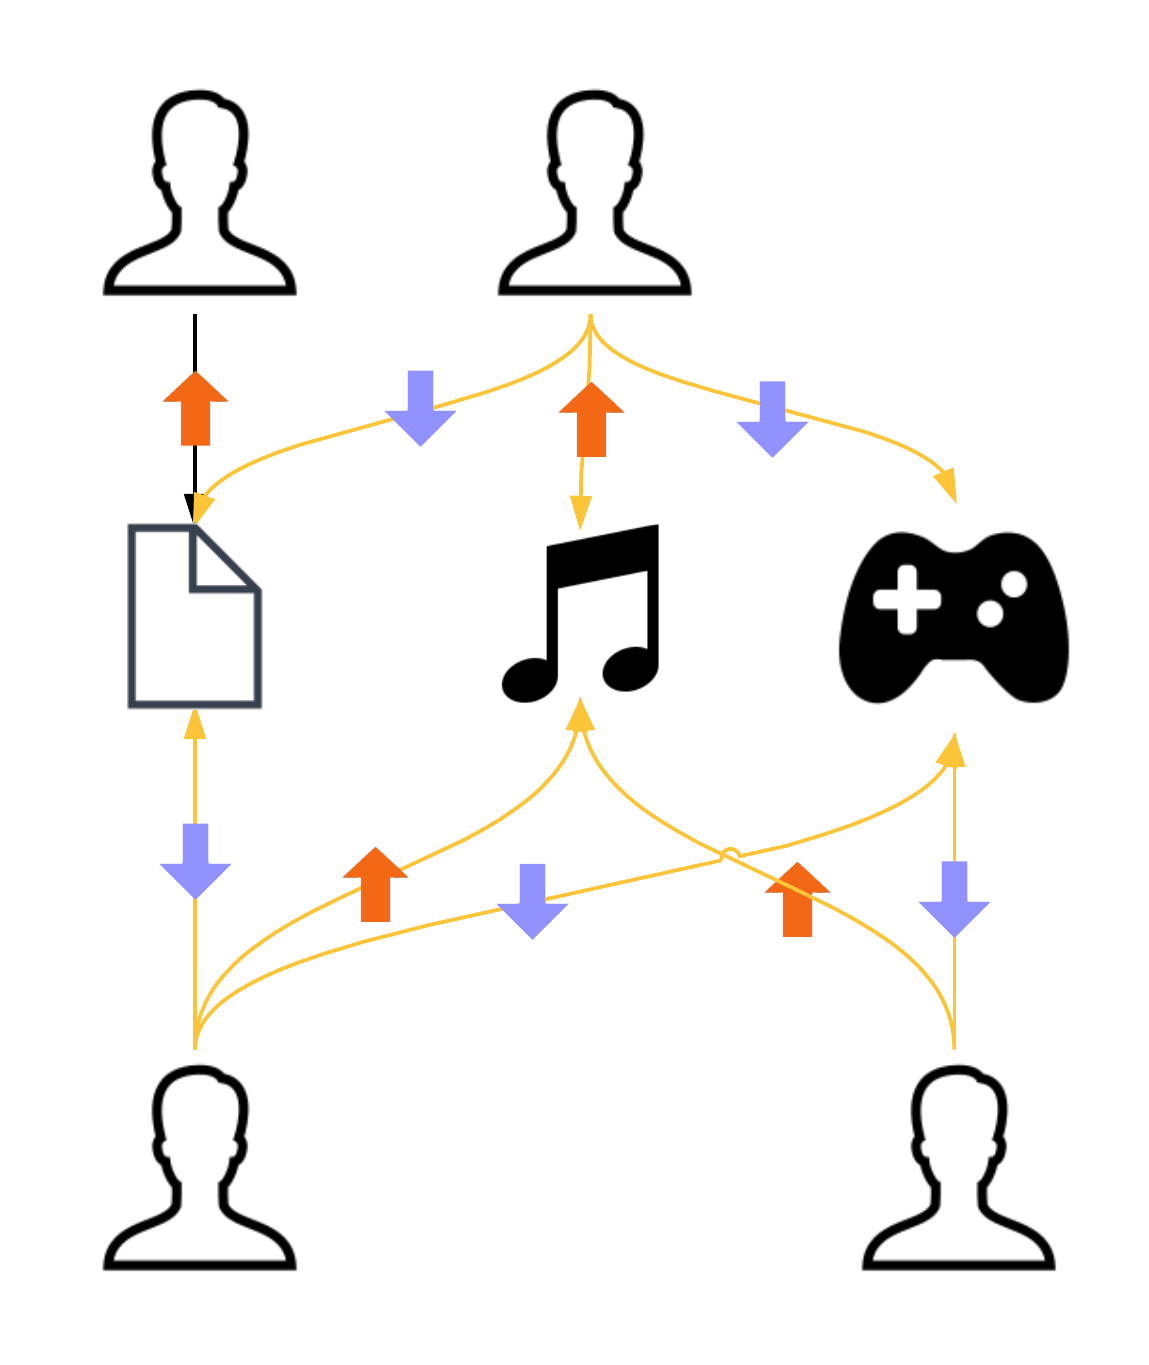
\includegraphics[width=\textwidth]{c-back_images/cf_2.png}
    \caption{After Prediction}
    \label{fig:cf2}
\end{subfigure}
\caption{Example of Collaborative Filtering}
\label{fig:cf}
\end{figure}

\subsection{Content Based Filtering}

\subsection{Hybrid Filtering}

The scope of this thesis lies in investigating the implications of comments and their content as a form of feedback.
\chapter{Dataset}

The dataset under observation is NU.nl, a popular Dutch online news website that comprises of predominantly Dutch comments scraped from their commenting platform NUjij.nl and spans over the year of 2014. An article is initially published on the original NU.nl site by editors, this is then shared by users and thereby receives comments through NUjij.nl.
\chapter{Investigations}
\label{chap:inv}
We perform preliminary investigations into assessing the dataset for later formulating the appropriate methodology that would best suit their innate properties.

\section{Attribution of Comments}
We seek an understanding of the strength of the association between comments and their authors. This would provide insight into user commenting behaviour, in particular whether a user has a unique vocabulary that distinguishes him from other users.

Authorship attribution aims at predicting the writer of a given a piece of text. In general a variety of stylometric and lexical features are used. Authorship attribution problems generally arise in forensic settings, and involve relatively long documents, and lists of possible authors limited to a few hundred candidate authors. Often, a sizable amount of example text is available for each candidate.In contrast, in our use case, the documents are short, the list of candidate authors is very large, and most are associated with little example text.                                          

\subsection{Literature}
Stamatatos provides an excellent summary of existing authorship attribution techniques \cite{stamatatos_survey_2009}. Most of the work discussed make use of both large documents and a smaller candidate author set. Stamatatos also points out that Support Vector Machines (SVM) perform extremely well as a distinguishing methodology in this particular scenario.

More recent work that looks into a smaller documents was done by Layton et al. \cite{layton_authorship_2010}, who look into authorship attribution for Twitter, where a micro-post (i.e., tweet) is restricted to 140 characters. Layton et al. opt for profile based feature representation of documents wherein all documents of a particular user are concatenated to form a super-document. They experiment with character $n$-grams with varying $n$ values and find that $4$-grams provide overall a good mean accuracy.

Work on large-scale attribution was carried out by Narayanan et al. \cite{narayanan_feasibility_2012}, who predict authors from a list of 100,000 candidate authors using a range of classifiers. Their dataset was comprised of blog posts, which are relatively longer than tweets or comments. They employed parts-of-speech tagging and a variety of lexical/character features for their purposes. A very interesting find in their work was that simple classifiers such as Naive Bayes and k-Nearest Neighbour performed better than SVM at the top ranks.

Our use case deals with shorter documents, namely comments, and a large candidate author set. We experiment with parts of methodologies adopted by Layton et al. \cite{layton_authorship_2010} and Narayanan et al. \cite{narayanan_feasibility_2012} as our problem is a combination of both. The upcoming sections discuss our methodology and the results of our experiments.

\subsection{k-NN Distance Based Attribution}
In our scenario, the training set is highly imbalanced, with a vast majority of authors having made very few comments and a handful of authors who made thousands of comments. For this reason, we adopt instance-based classification, wherein each document contributes on its own to the attribution and choose a simple 1-NN classifier.

For a given comment, we predict the nearest most resembling comment in the training set. It is to be noted that we do not make profile based predictions by grouping all comments of a single user together but rather each comment constitutes its own class. The overall framework is illustrated in Figure~\ref{fig:inv_1}.

\begin{figure}[!h]
\centering
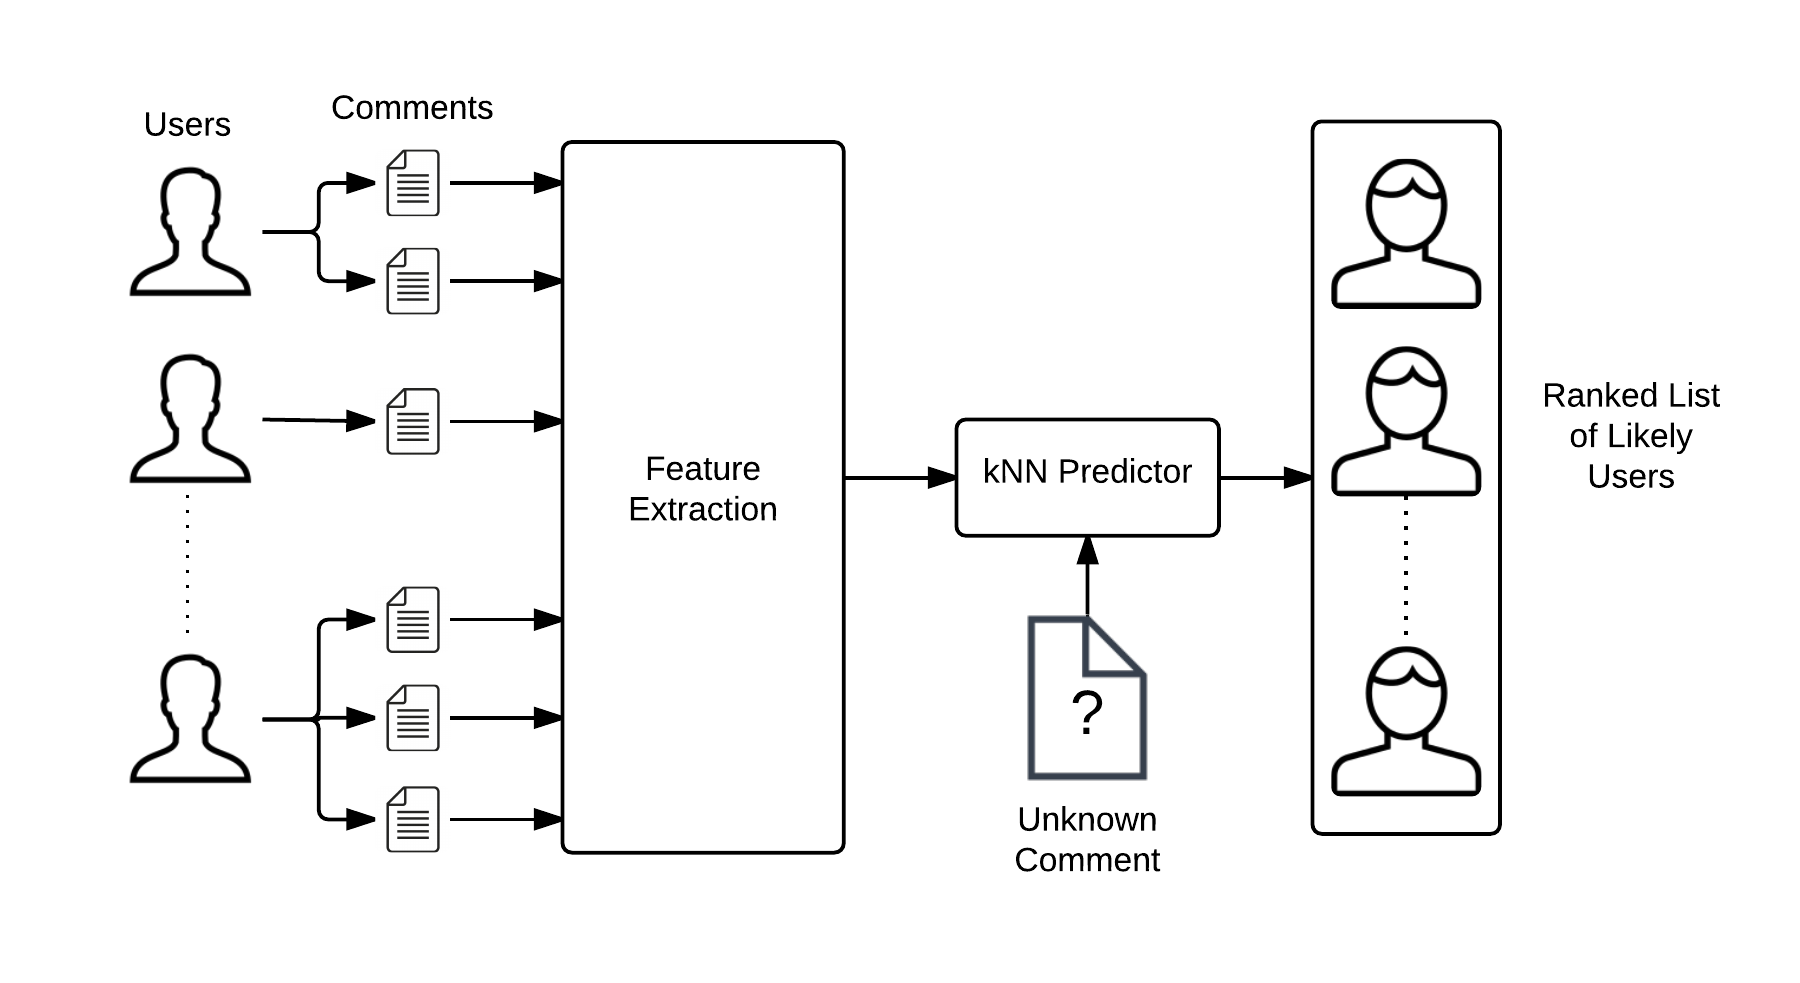
\includegraphics[width=1\textwidth]{c-inv_images/inv_1.png}
\caption{Authorship Attribution}
\label{fig:inv_1}
\end{figure}

The features we make use of are the character $n$-grams similar to that of Layton et al., since our use case also deals with similar informal text and shorter documents. We experiment with different values of $n$. We expect the value of $n$ to be important, since our data set is not homogeneously mono-lingual. We perform basic thresholding by selecting only those $n$-grams that occur more than five times in the entire dataset.

The character $n$-grams are converted into \textit{tf-idf} weight vectors, \textit{tf-idf} weights are essentially the product of the term frequency in a single document and the inverse document frequency. It aids in discerning the unique terms in a document thereby would directly expose user-specific features. Tf-idf is generally formulated as,

\begin{align*}
tfidf &= f_{t,d} * log\frac{N}{n_t}\\
\text{where, }& f_{t,d} \text{ - frequency of term $t$ in document $d$}\\
& N \text{ - total documents in corpus}\\
& n_t \text{ - number of documents with term $t$}
\end{align*}

Each vector represents a single comment and if a particular $n$-gram is not present then the corresponding \textit{tf-idf} entry is zero in that index. We experiment with two different distance functions as a means for finding their nearest neighbours. Namely, euclidean distance similar to what Narayanan et al. \cite{narayanan_feasibility_2012} used and cosine similarity. If $p_i$ and $q_i$ are two vectors then we formulate,

\begin{align*}
\text{Eucildean Distance} &= ||(q-p)||\\
\text{Cosine Similarity} &= \frac{p.q}{||p||*||q||}\\
\text{where, }||x|| &= \sqrt{x_1^2 + x_2^2 + x_3^ + ... + x_n^2} \text{ is the norm of the vector }x\\
\end{align*}

Euclidean distance directly measures the magnitude of the distance between the two vectors whereas cosine similarity measures the directional difference between the two vectors. 

\subsection{Attribution Experiments}
NU.nl comments are strictly moderated and the possibility of occurrence of spam is low, therefore we take the comments in their original form for $n$-gram tokenization without any form of filtering. The entire dataset encompasses over the last three months of 2014 as previously discussed in Chapter~\ref{chap:data}.

We partition the data temporally: the first 10 days of comments are taken as the training set and the next 3 days as the test set, we slide this 10-3 day split over the entire dataset, resulting in total of 79 samples of the data. Figure~\ref{fig:inv_2} better represents the sampling strategy.

\begin{figure}[!h]
\centering
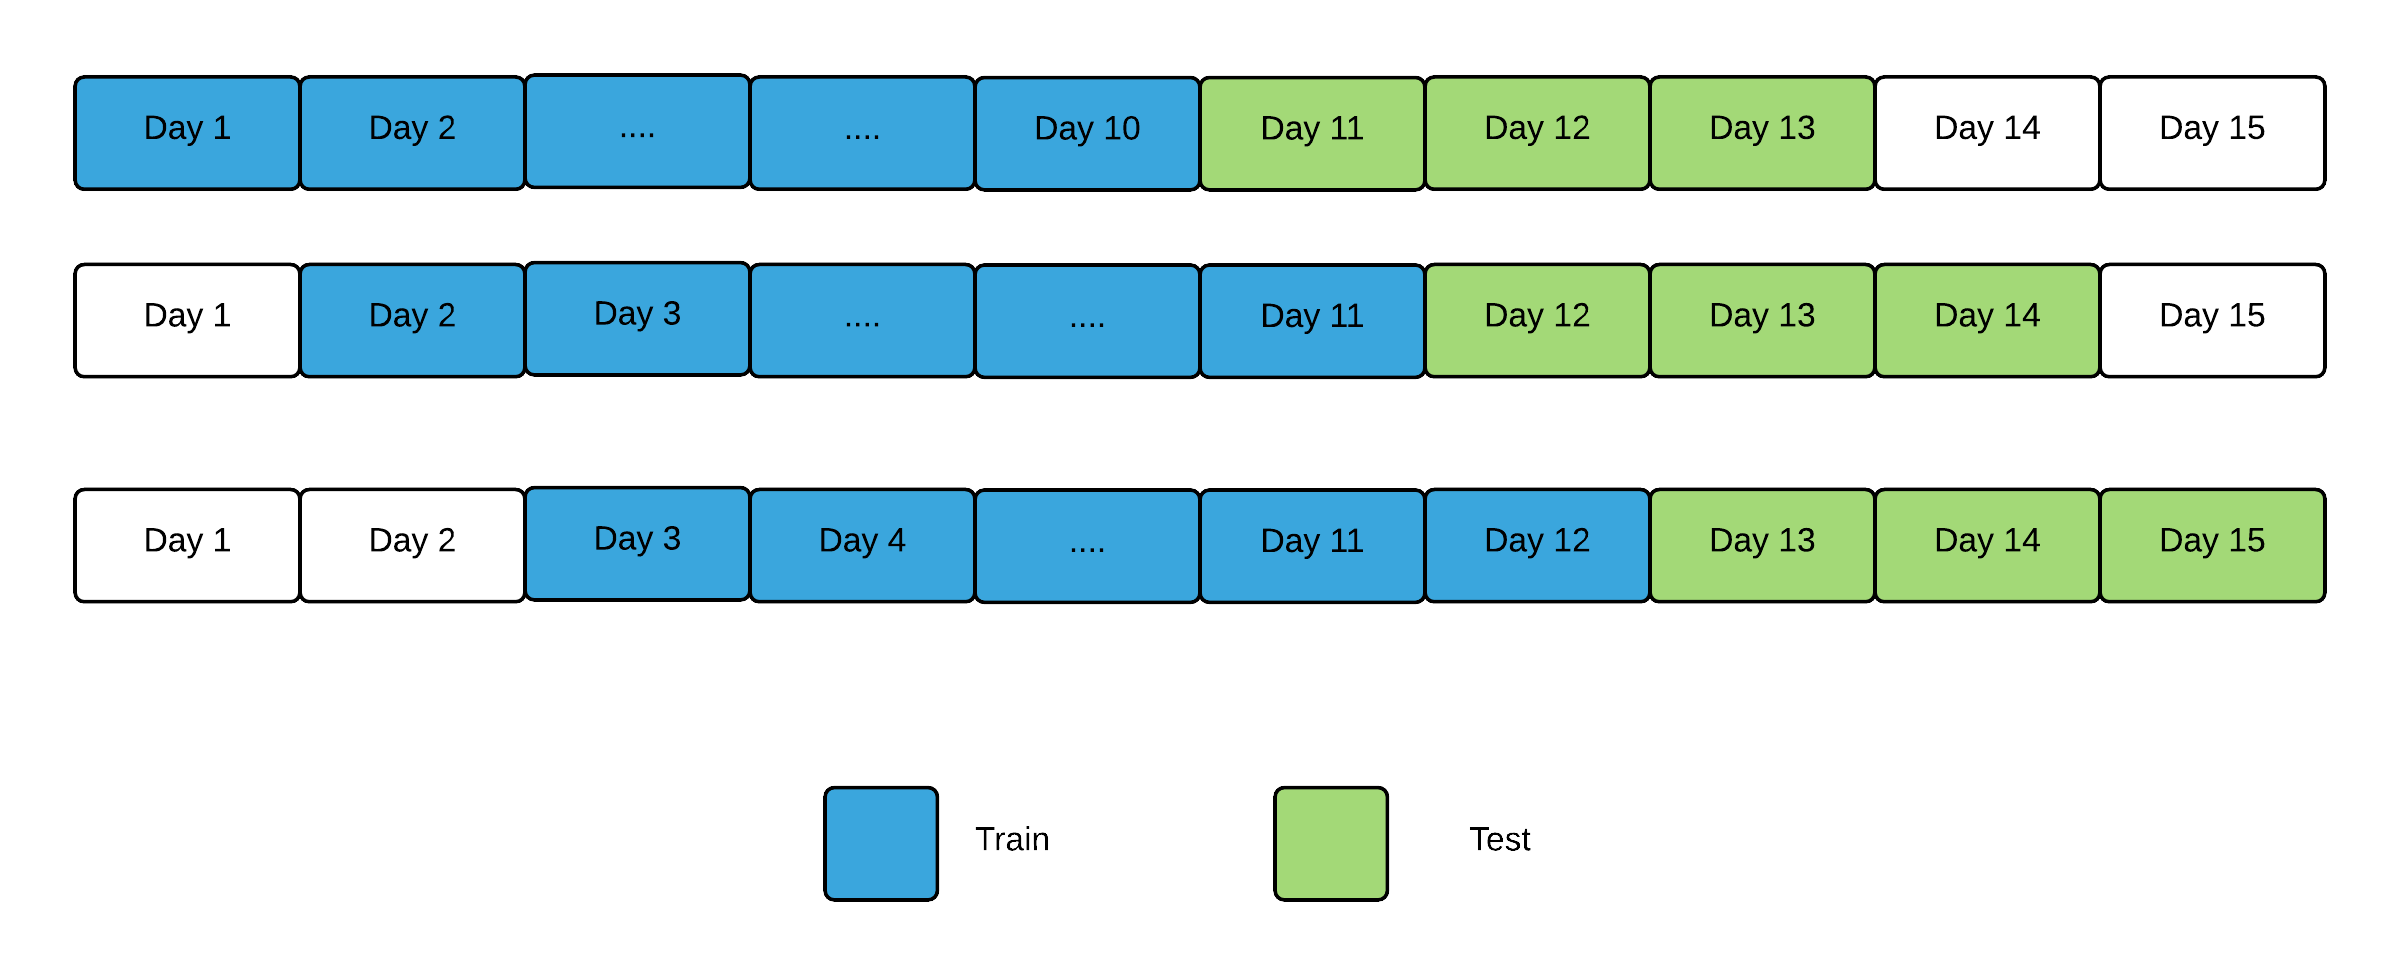
\includegraphics[width=1\textwidth]{c-inv_images/inv_2.png}
\caption{Sampling}
\label{fig:inv_2}
\end{figure}

This strategy was chosen since we are interested in predicting authorship based on historical data, and in any real world scenario, one can only predict future behaviour based on past instances and not the other way around. 

We also take into consideration only the candidate authors who had made at-least three comments, since we assume that it is not possible to make predictions with less data. Table~\ref{tab:split} shows the underlying split of the data averaged over all the samples.

\begin{table}[!h]
\centering
\begin{tabular}{|c|c|c|c|}
\hline
 \textbf{Train/Test} & \textbf{Average Users} & \textbf{Average Items} & \textbf{Average Comments} \\ \hline
 Train & 3930.55 & 1267.42 & 27275.09 \\ \hline
 Test & 3910.33 & 461.07 & 10356.82 \\ \hline
\end{tabular}
\caption{Data Split}
\label{tab:split}
\end{table}

The metric we use for evaluation is Mean Reciprocal Rank (MRR) which is %essentially 
the average of the reciprocal rank of the first hit in the list of candidates. We compute RR for those instances in which the author is found in the top 100 ranked results. For the rest of the cases, we assume that the author was ranked at infinity, and these cases contribute a RR of zero to the MRR. We also make use of $MAP@N$ which represents the mean average precision upto rank N.

As a sanity check, we calculated a trivial baseline that drew a comment from the training set at random. In essence, the baseline prioritizes users who have made more comments. The baseline had an $MRR < 0.001$ in both cases of NU and SC.

Table~\ref{tab:com_results} shows the results of classification averaged over all comments. 

\begin{table}[!h]
\centering
\begin{tabular}{|l|c|c|c|c|}
\hline
 \textbf{Distance Measure} & \textbf{n-gram} & \textbf{MRR} & \textbf{MAP@5} & \textbf{MAP@10}\\ \hline
 \multirow{3}{*}{Euclidean}& 2 & & & \\ \cline{2-5}
 & 3 & 0.0305 & 0.0141 & 0.0163 \\ \cline{2-5}
 & 4 & & & \\ \hline
 \multirow{3}{*}{Cosine} & 2 & &  & \\ \cline{2-5}
 & 3 & 0.0711 & 0.0357 & 0.0412 \\ \cline{2-5}
 & 4 & & & \\ \hline
\end{tabular}
\caption{Per-Comment Results}
\label{tab:com_results}
\end{table}

Clearly, the cosine similarity based prediction outperforms the euclidean distance based prediction. This may be due to the fact that cosine similarity outright ignores vectors which are entirely dissimilar whereas the euclidean distance measure does not. In the case of text, dissimilar vectors directly imply two pieces of text with entirely different words, this better suits our goal of trying to find similar comments.

But, it is open to question whether authorship attribution utilizing cosine similarity for all domains would outperform euclidean distance. Narayanan et al. \cite{narayanan_feasibility_2012} had used Euclidean distance for the special case of blogs which are much larger than comments and also a different set of features.

Considering the scale of results for our classification task wherein there were potentially around 4k different users to attribute to, we were able to make a prediction on average in the top 15 ranks. This implies that users of NU.nl more or less utilize the same words over time that makes them uniquely identifiable.

If one were to make use of conventional authorship features such as text compression, parts-of-speech, lexical features (frequency of punctuation, word length, sentence length), which capture subtle stylometric features rather than just the text, one might see an improvement over the base performance. But, use of such features is out of scope in this work. 

In the end we were still able to make decent predictions even without such advanced features and were able to assess that the average user of NU.nl utilizes the same vocabulary over time.

->TODO INSERT RANK GRAPHS

We also look into the stability of the predictions over different conditions so as to determine whether it is biased towards a particular nature of the dataset.

All plots are essentially histograms averaged with respect to the particular X-axis metric. Due to the wide variations that would potentially occur due to the wide range in the actual number of instances in each bin, we utilize Quantile Bounded Mean (QBM) as an approximation towards the trend of the plot.

To calculate the QBM approximation, we split our dataset that is binned with respect to the X-axis metric then split into 5\% quantiles. We then find the average over these quantiles resulting in a single data point for that quantile, connecting all such data points finally results in a smoothed approximation of the trend of the plot. We do not take into account the last quantile as it would contain potential outliers that are not characteristic of the entire dataset.

\begin{figure}[!h]
\centering
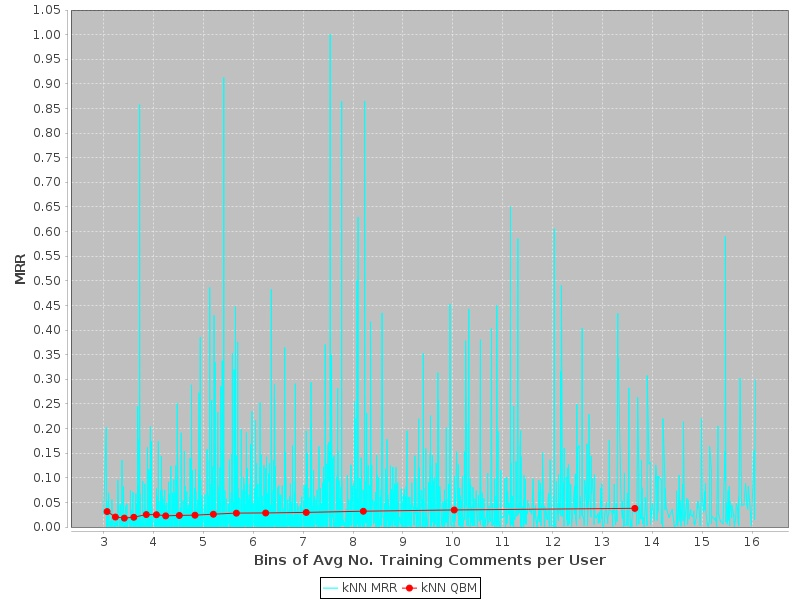
\includegraphics[width=0.75\textwidth]{c-inv_images/AuthorshipUserCountMRR.jpeg}
\caption{MRR Predictions vs No. Training Comments}
\label{fig:AuthorshipUserCountMRR}
\end{figure}

Figure~\ref{fig:AuthorshipUserCountMRR} is a plot of the MRR predictions versus the number of training comments that were utilized. As can be seen most of the instances occurred from 3-5 training comments, there is a slight fall between 3 and 4 but it picks up after 4 and generally stabilizes from there on. It is also to be noted that there are no drastic changes towards the end implying that more comments do not immediately imply better predictions. This also yields insight into the least number of comments required to make predictions - in this case 4 seems to be a good least threshold.

\begin{figure}[!h]
\centering
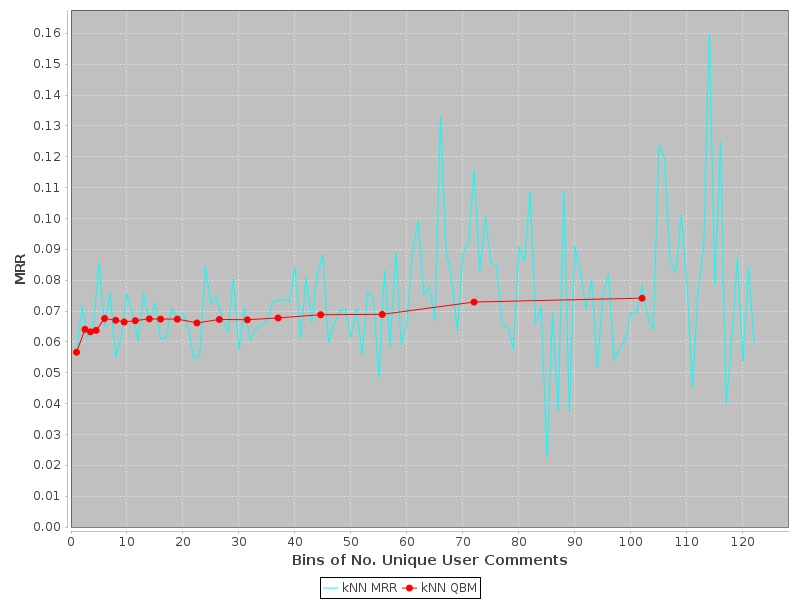
\includegraphics[width=0.75\textwidth]{c-inv_images/AuthorshipItemCountMRR.jpeg}
\caption{MRR Predictions vs No. Unique Users who Commented}
\label{fig:AuthorshipItemCountMRR}
\end{figure}

Figure~\ref{fig:AuthorshipItemCountMRR} is a plot of the MRR predictions versus the number of unique users who had commented on the item. This measure is essentially a surrogate of the popularity of the item - the more the unique users who commented the more popular the item is expected to be. There is a slight increase as the number of unique users increases - with a significant rise from 1 - 2 unique users and generally it stabilizes after 7 with slight increases towards the end. Yet again there are no drastic changes as observed previously.


\begin{figure}[!h]
\centering
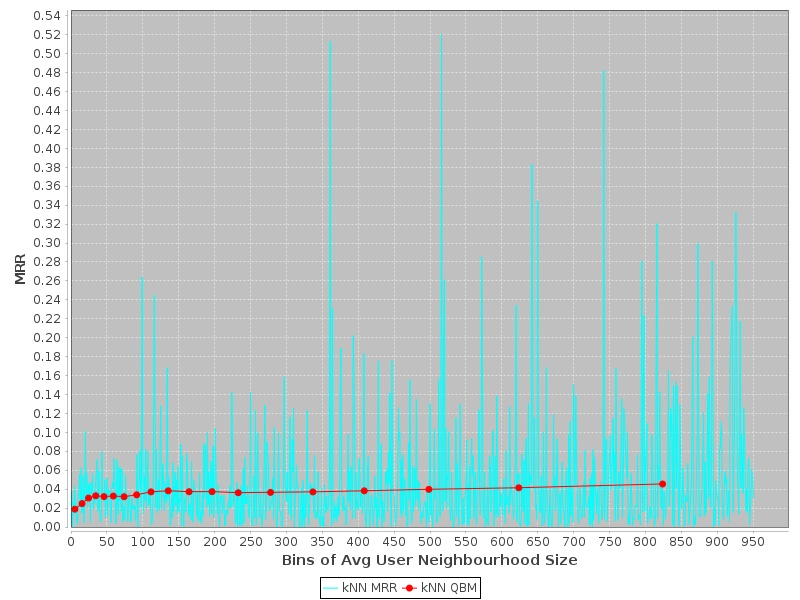
\includegraphics[width=0.75\textwidth]{c-inv_images/AuthorshipUserNeighMRR.jpeg}
\caption{MRR Predictions vs Neighbourhood Size of User}
\label{fig:AuthorshipUserNeighMRR}
\end{figure}

Figure~\ref{fig:AuthorshipUserNeighMRR} is a plot of the MRR predictions versus the user neighbourhood sizes. The user neighbourhood is simply computed by the sum of the unique users who co-commented along with the target user. The average neighbourhood size per user of the entire dataset was found to be 460.89 users. The MRR stabilizes after a neighbourhood size of ~30 implying that users who comment on items that are more often commented by other users are better attributed. But, similar to previous observations there are no drastic changes.

We further investigate the co-commenter behaviour by utilizing the target user's neighbourhood users' labels as the ground truth rather than only the target user's label. We utilize cosine distance for our predictions as we had previously observed that cosine distance performed better. Table~\ref{tab:co_com_results} shows the results of the co-commenter classification.

\begin{table}[!h]
\centering
\begin{tabular}{|l|c|c|c|c|}
\hline
 \textbf{(TODO ENTIRE DATASET) Predictor} & \textbf{n-gram} & \textbf{MRR} & \textbf{MAP@5} & \textbf{MAP@10}\\ \hline
 \multirow{3}{*}{k-NN Cosine} & 2 & &  & \\ \cline{2-5}
 & 3 & 0.3472 & &  \\ \cline{2-5}
 & 4 & & & \\ \hline
 \multirow{3}{*}{Random} & 2 & &  & \\ \cline{2-5}
 & 3 & 0.2150 & &  \\ \cline{2-5}
 & 4 & & & \\ \hline
\end{tabular}
\caption{Per-Comment Co-Commenter Results}
\label{tab:co_com_results}
\end{table}

A surprising observation was that random predictions perform close to that of our k-NN predictions. This is characteristic of the neighbourhood size - as we previously observed that the average neighbourhood size was 460.89 per user, considering this with the average number of users as seen in Table~\ref{tab:split}, in an ideal world scenario there would be ~9 clusters of users who comment on articles. Thereby it takes simply to find 1 of the 9 clusters to make a prediction.

As before, we investigate particular properties of the dataset and their influence on our predictions.

\begin{figure}[!h]
\centering
\begin{subfigure}[b]{0.475\textwidth}
    \centering
    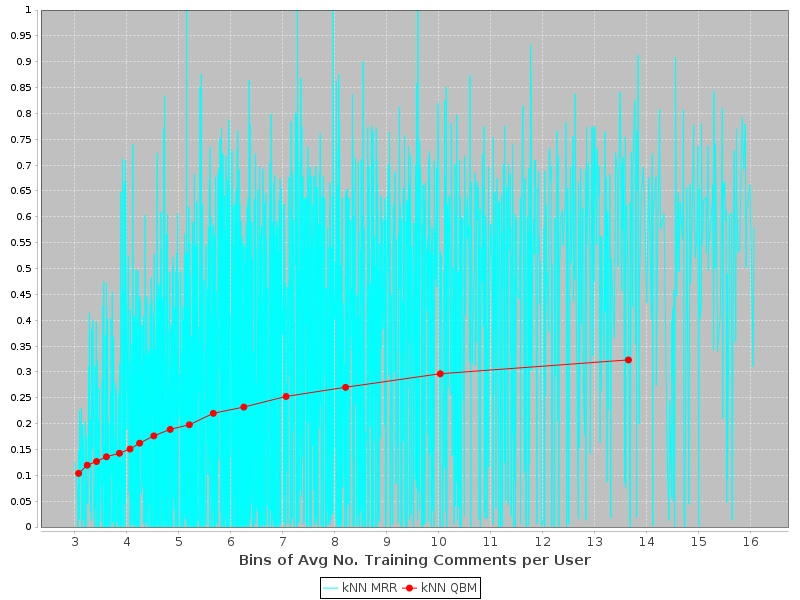
\includegraphics[width=\textwidth]{c-inv_images/co_AuthorshipUserCountMRR.jpeg}
    \caption{Cosine k-NN}
\end{subfigure}
\begin{subfigure}[b]{0.475\textwidth}
    \centering
    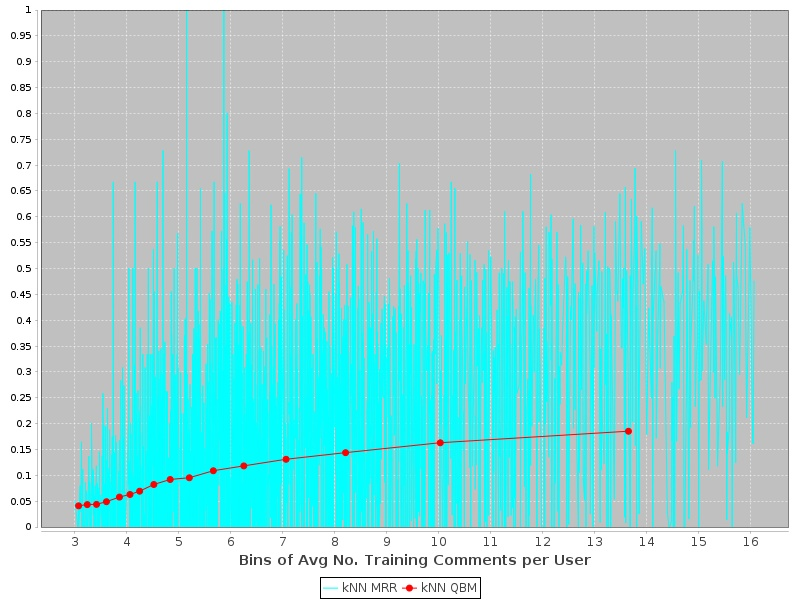
\includegraphics[width=\textwidth]{c-inv_images/randCo_AuthorshipUserCountMRR.jpeg}
    \caption{Random}
\end{subfigure}
\caption{Co-Commenter MRR Predictions vs No. Training Comments}
\label{fig:co_AuthorshipUserCountMRR}
\end{figure}

Figure~\ref{fig:co_AuthorshipUserCountMRR} is a plot of the co-commenter MRR predictions versus the number of training comments that were utilized. Both cosine k-NN and random predictions observe the same trend of gradual increase as the number of comments increases as increase in number of comments potentially increases the size of the ground truth labels under consideration.

\begin{figure}[!h]
\centering
\begin{subfigure}[b]{0.475\textwidth}
    \centering
    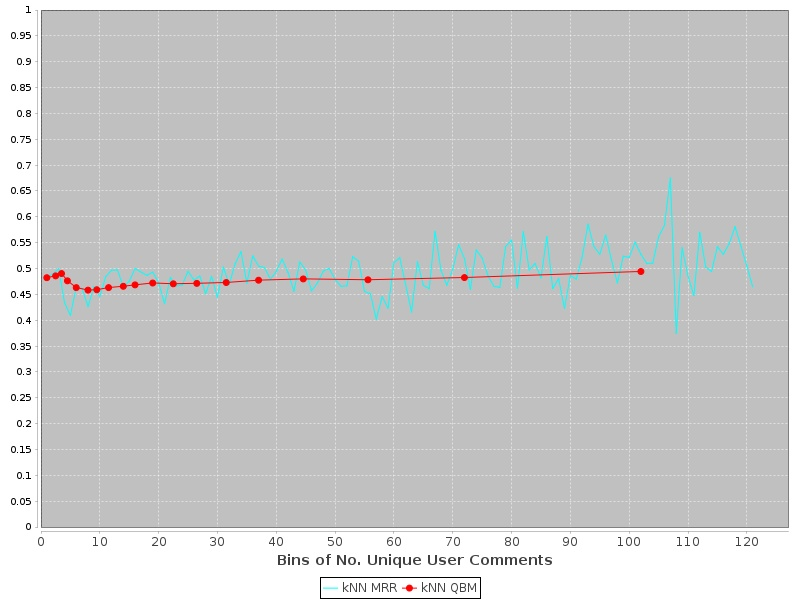
\includegraphics[width=\textwidth]{c-inv_images/co_AuthorshipItemCountMRR.jpeg}
    \caption{Cosine k-NN}
\end{subfigure}
\begin{subfigure}[b]{0.475\textwidth}
    \centering
    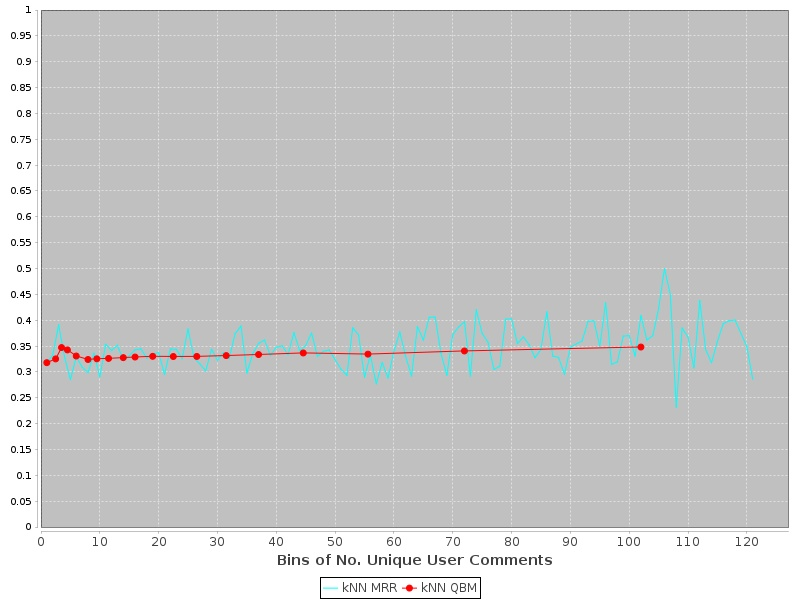
\includegraphics[width=\textwidth]{c-inv_images/randCo_AuthorshipItemCountMRR.jpeg}
    \caption{Random}
\end{subfigure}
\caption{Co-Commenter MRR Predictions vs No. Unique Users who Commented}
\label{fig:co_AuthorshipItemCountMRR}
\end{figure}

Figure~\ref{fig:co_AuthorshipItemCountMRR} is a plot of the MRR predictions versus the number of unique users who had commented on the item. Only earlier on, there is a slight rise and a subsequent fall whereas the rest is stabilized. This might be an indication that users with very large neighbourhood sizes comment on the least popular articles thereby causing a slight rise whereas the medium popular that ranges from ~7 are commented by the average user.

\begin{figure}[!h]
\centering
\begin{subfigure}[b]{0.475\textwidth}
    \centering
    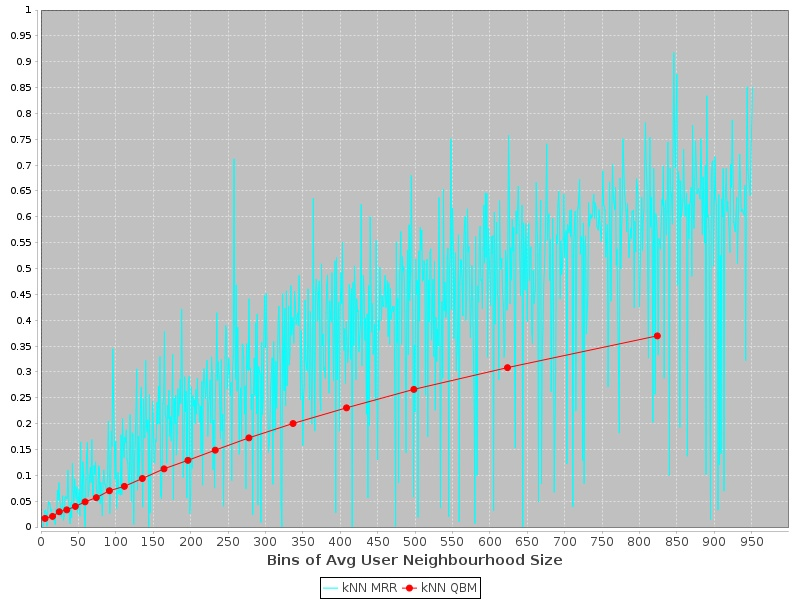
\includegraphics[width=\textwidth]{c-inv_images/co_AuthorshipUserNeighMRR.jpeg}
    \caption{Cosine k-NN}
\end{subfigure}
\begin{subfigure}[b]{0.475\textwidth}
    \centering
    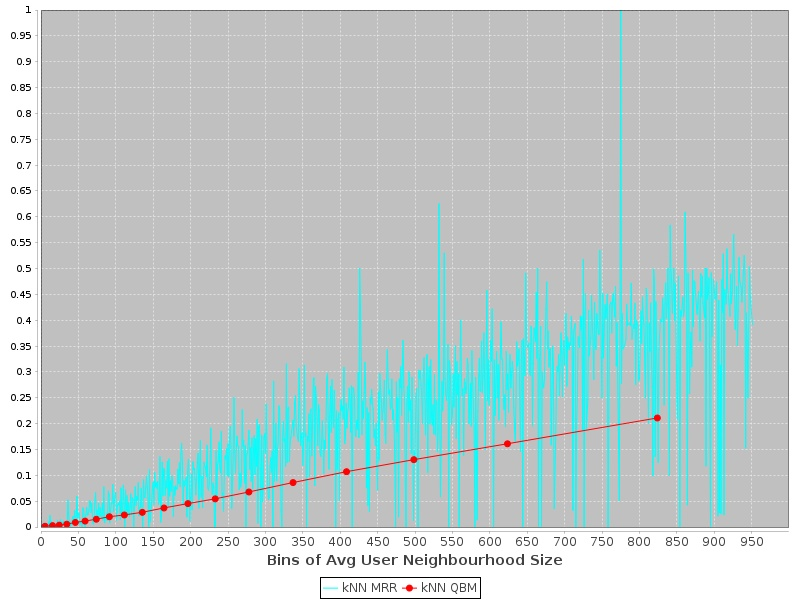
\includegraphics[width=\textwidth]{c-inv_images/randCo_AuthorshipUserNeighMRR.jpeg}
    \caption{Random}
\end{subfigure}
\caption{Co-Commenter MRR Predictions vs Neighbourhood Size of User}
\label{fig:co_AuthorshipUserNeighMRR}
\end{figure}

Figure~\ref{fig:AuthorshipUserNeighMRR} is a plot of the MRR predictions versus the user neighbourhood sizes. This without a doubt shows the anticipated that as the neighbourhood size increases, the number of ground truth labels increase and subsequently the MRR increases.

\subsection{Inferences}
In conclusion, we were able to make decent predictions for single label attribution even with simple features. For full fledged authorship attribution, one might employ the technique used here as a sampling strategy to narrow down a large number of authors to a candidate set that then later undergoes the entire process utilizing stylometric features for accurate prediction.

The co-commenter prediction shows the innate nature of the dataset wherein it is largely clustered into groups of users who consistently co-comment on the same set of items. Thereby potentially showing that collaborative filtering could be a good predictor in finding the items the target user would comment on. In addition, the accuracy of the single label attribution also encourages us to model the user by his unique vocabulary thereby use that as an indication of the user and not necessarily utilize the user's explicit label/id.
\chapter{Method (draft)}
\label{chap:method}
In this chapter, we discuss the proposed methodology by describing the employed recommender framework and the different algorithms that are plugged into it.

\section{Framework (TODO - insert references)}
Due to the infeasibility of deploying a live recommender on NU.nl, we opt for offline evaluation that simulates the online environment. In an online scenario, the query for a recommendation is generated every time the user logs in or whenever a user views a news article. But, this implicit data is absent and what we posses are the comments as interactions.

Therefore, one crucial assumption we make is that the moment the user comments is the moment he queried for a recommendation. So we consider the brief time period before a comment is when a query for recommendations was made. We had also previously reported in Chapter~\ref{chap:data} that the average span between the time of article publication and the last comment was close to 32 hours (TODO-cross check). This in a simple way, is an indicator of how far back we must look and what would be considered as fresh. We go into much more detail regarding freshness in this scenario in Section~ (TODO- insert section). These fresh items are then treated as the candidate items for our recommender.

To summarize, for each comment we would retrieve the recent articles before the comment's time point then rank them through our recommender and verify if the target item is in the top of our ranked list of items. The model of the recommender itself is trained over the interactions preceding the comment's time point. We investigate how far back to look for training the model in Section~ (TODO- insert section). Figure~\ref{fig:frame} illustrates the recommender framework.

\begin{figure}[!h]
\centering
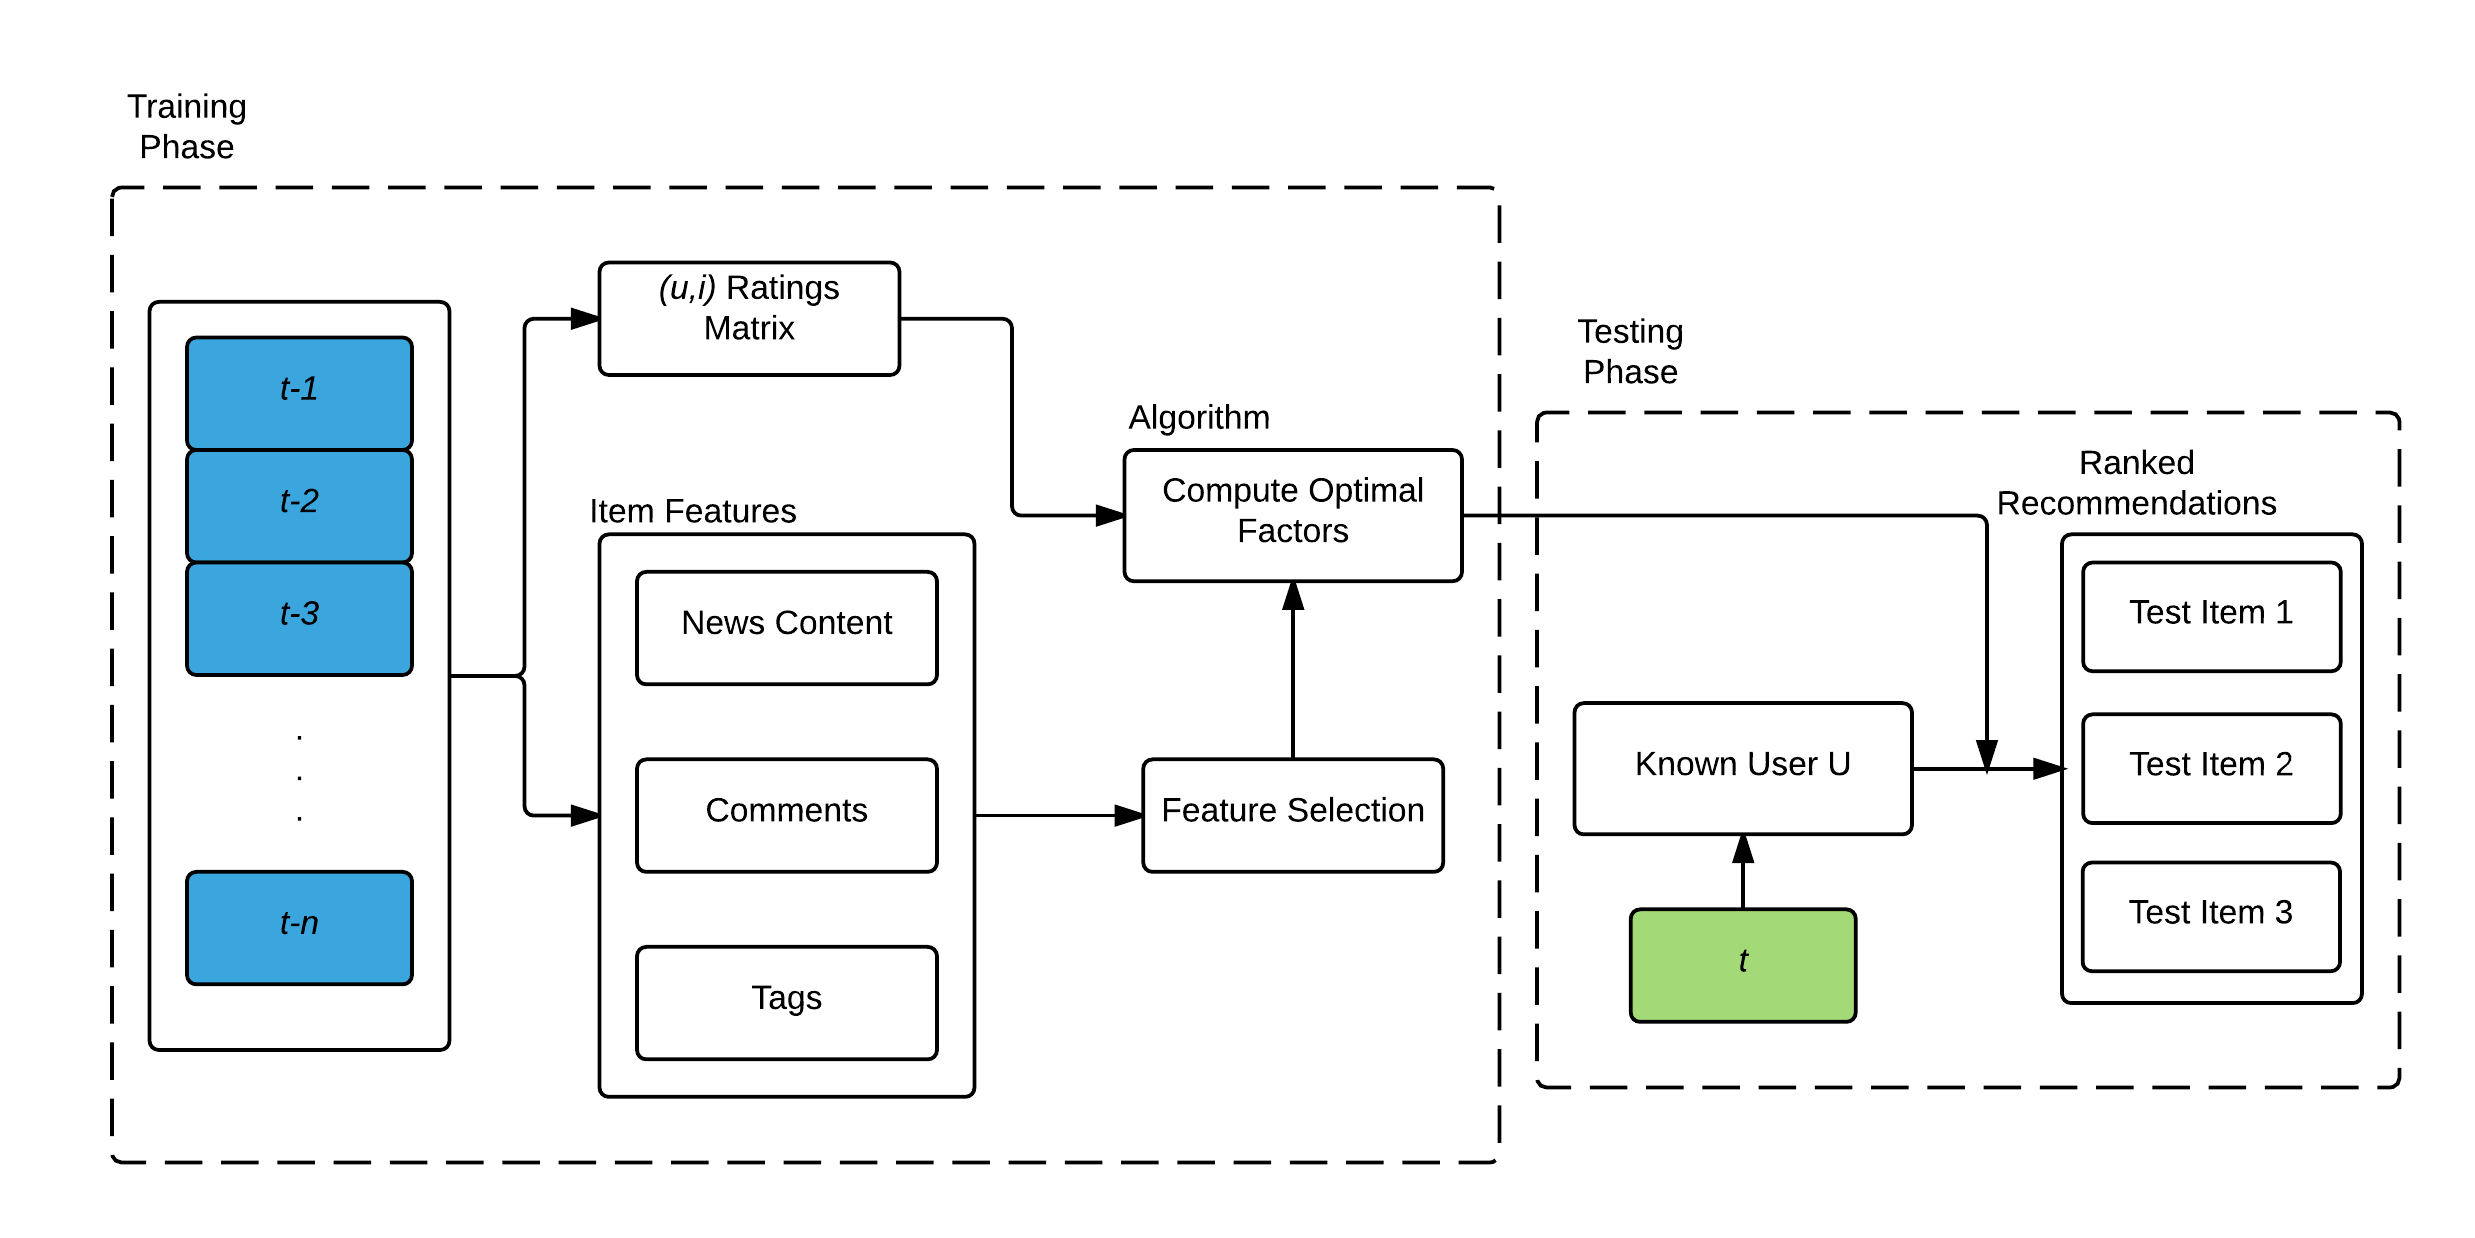
\includegraphics[width=0.85\textwidth]{c-method_images/frame.png}
\caption{Framework}
\label{fig:frame}
\end{figure}

\section{Feature Engineering}

\section{Algorithm}
\cite{rendle_factorization_2012}
\subsection{SVD++}
\cite{koren_factorization_2008}
\subsection{gSVD++}
\cite{manzato_gsvd++:_2013}


\chapter{Evaluation}
\chapter{Conclusion and Outlook}

%% Use letters for the chapter numbers of the appendices.
%\appendix

%\chapter{TODO}


\bibliography{report}

\end{document}